\documentclass[pdf]{beamer}
\mode<presentation>{}
\usetheme{Dresden}
\usepackage{apalike}
%% preamble
\title{Numerically solving the 1D Serre Equations In the Presence of Discontinuities}
\author{Jordan Pitt, Stephen Roberts and Christopher Zoppou}

\begin{document}
%% title frame
\begin{frame}
\titlepage
\end{frame}
%% normal frame
\section{Serre Equations}
\subsection{}

\begin{frame}{Serre Equations}
\begin{subequations}\label{eq:Serre_conservative_form}
\begin{gather*}
\dfrac{\partial h}{\partial t} + \dfrac{\partial (uh)}{\partial x} = 0,
\label{eq:Serre_continuity}
\end{gather*}
\begin{gather*}
\underbrace{\underbrace{\dfrac{\partial (uh)}{\partial t} + \dfrac{\partial}{\partial x} \left ( u^2h + \dfrac{gh^2}{2}\right )}_{\text{Shallow Water Wave Equations}} + \underbrace{\dfrac{\partial}{\partial x} \left (  \dfrac{h^3}{3} \left [ \dfrac{\partial u }{\partial x} \dfrac{\partial u}{\partial x} -u \dfrac{\partial^2 u}{\partial x^2}  - \dfrac{\partial^2 u}{\partial x \partial t}\right ] \right )}_{\text{Dispersion Terms}} = 0}_{\text{Serre Equations}}
\label{eq:Serre_momentum}
\end{gather*}
\end{subequations}
\end{frame}

\begin{frame}{Conservation Law Form}
New conserved quantity
\begin{gather}\label{eq:Gdefinition}
G = uh - h^2 \dfrac{\partial h}{\partial x} \dfrac{\partial u}{\partial x} - \frac{h^3}{3} \dfrac{\partial^2 u}{\partial x^2}.
\end{gather}
Reformulated equations
\begin{subequations}
\begin{gather}
\dfrac{\partial h}{\partial t} + \dfrac{\partial (uh)}{\partial x} = 0
\label{eq:Serrecon_continuity}
\end{gather}
\begin{gather}
\dfrac{\partial G}{\partial t} + \dfrac{\partial}{\partial x}\left(Gu + \dfrac{gh^2}{2} - \dfrac{2h^3}{3}\dfrac{\partial u}{\partial x}\dfrac{\partial u}{\partial x}\right) = 0
\label{eq:Serrecon_momentum}
\end{gather}
\label{eq:Serrecon}
\end{subequations}
\end{frame}

\section{Finite Difference Finite Volume Methods}
\subsection{Description}

\begin{frame}{Basic Overview}
Vector of conserved quantities:
\[\boldsymbol{U} = 
\left[
\begin{array}{c}
h \\
G							
\end{array} \right] \]

Algorithm:
\[\mathcal{H}\left(\boldsymbol{\bar{U}}^n,\Delta x ,\Delta t \right) = \left\lbrace 
\begin{array}{c c c} 
	\boldsymbol{U}^n &=& \mathcal{M}\left(\boldsymbol{\bar{U}}^n\right) \\
	\boldsymbol{u}^n &=& \mathcal{A}\left(\boldsymbol{U}^n, \Delta x\right) \\
	\boldsymbol{\bar{U}}^{n+1} &=& \mathcal{L}\left(\boldsymbol{\bar{U}}^{n},\boldsymbol{u}^n, \Delta x ,\Delta t\right)							
\end{array} \right. .\]
\end{frame}

\begin{frame}{$\mathcal{A}$ : elliptic equation for $G$}

Subscripts represent the spatial cell centre and superscripts represent the time step.

\[\boldsymbol{u}^n = \left[u_0^n ,u_1^n , \dots , u_m^n\right]\]

where $x_i - x_{i-1} = \Delta x$ for all $i$. 

\[	\boldsymbol{u}^n = \mathcal{A}\left(\boldsymbol{U}^n, \Delta x\right) \]
In this version of the scheme this represents an appropriate order centered finite difference approximation to \eqref{eq:Gdefinition}.
\end{frame}

\begin{frame}{$\mathcal{L}$ : conservative update}
Bar represents the average over the cell so for example

\[\bar{u}^n_i = \frac{1}{\Delta x}\int_{x_i - \frac{\Delta x}{2}}^{x_i + \frac{\Delta x}{2}} u(x,t^n) dx\]



\[\boldsymbol{\bar{U}}^{n+1} = \mathcal{L}\left(\boldsymbol{\bar{U}}^{n},\boldsymbol{u}^n, \Delta x ,\Delta t\right)\]

This represents an appropriate order Godunov type finite volume method. In particular we use the the method by Kurganov \cite{Kurganov-etal-2001-707}.

%\[ u - \sqrt{gh}\le \upsilon_p \le u + \sqrt{gh}\]
\end{frame}

\begin{frame}{$\mathcal{M}$ : nodal values to cell averages}
\[
	\boldsymbol{U}^n = \mathcal{M}\left(\boldsymbol{\bar{U}}^n\right) \]
For first and second order versions this is the identity map.
\end{frame}


\begin{frame}{$\mathcal{H}$ : Euler step}
\[\mathcal{H}\left(\boldsymbol{\bar{U}}^n,\Delta x ,\Delta t \right) = \left\lbrace 
\begin{array}{c c c} 
	\boldsymbol{U}^n &=& \mathcal{M}\left(\boldsymbol{\bar{U}}^n\right) \\
	\boldsymbol{u}^n &=& \mathcal{A}\left(\boldsymbol{U}^n, \Delta x\right) \\
	\boldsymbol{\bar{U}}^{n+1} &=& \mathcal{L}\left(\boldsymbol{\bar{U}}^{n},\boldsymbol{u}^n, \Delta x ,\Delta t\right)							
\end{array} \right. .\]

Need to use strong stability preserving Runge-Kutta \cite{Gottlieb-etal-2009-251} steps to increase the order of accuracy in time.
\end{frame}

\section{Validation}
\subsection{Analytic Validation}

\begin{frame}{Soliton}
\begin{subequations}
\begin{gather}
h\left(x,t\right) = a_0 + a_1\text{sech}^2\left( \kappa\left(x - ct\right)\right)
\end{gather}
\begin{gather}
u\left(x,t\right) = c\left(1 - \dfrac{a_0}{h(x,t)} \right)
\end{gather}
\begin{gather}
\kappa = \dfrac{\sqrt{3a_1}}{2a_0 \sqrt{ a_0 + a_1}}
\end{gather}
\begin{gather}
c = \sqrt{g \left(a_0 + a_1\right)}
\end{gather}
\label{eq:sol}
\end{subequations}
Nonlinearity ($\eta$):
\[\eta = \frac{a_1}{a_0}\]
\end{frame}

%\begin{frame}{Experiment 1}
%$a_0 = 10.0\text{m}$ , $a_1 = 1.0\text{m}$ ($\eta = 0.1$) , $\Delta x = 100 /2^{6}\text{m} = 0.15625 \text{m}$, $\Delta t = \frac{0.5}{\sqrt{g (a_0 + a_1)}} \Delta x \; \text{s}$

%First Order:

%\begin{figure}
%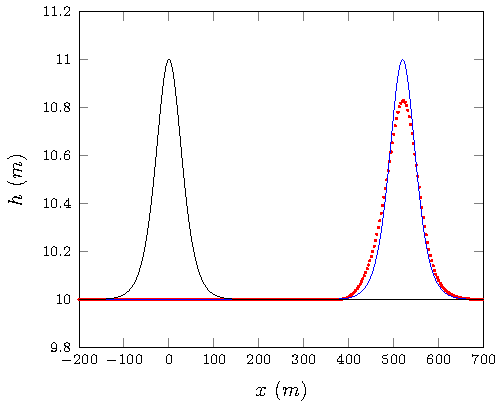
\includegraphics[width=5.0cm]{../pictures/soliton/lownonling10/ex/o1plotsolh-figure0.pdf}
%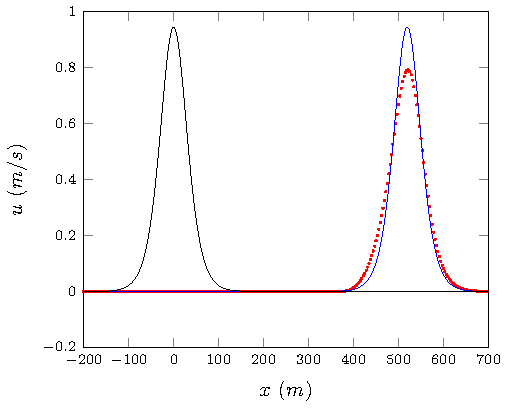
\includegraphics[width=5.0cm]{../pictures/soliton/lownonling10/ex/o1plotsolu-figure0.pdf}
%\end{figure}
%\end{frame}

%\begin{frame}{Experiment 1}
%Second Order:

%\begin{figure}
%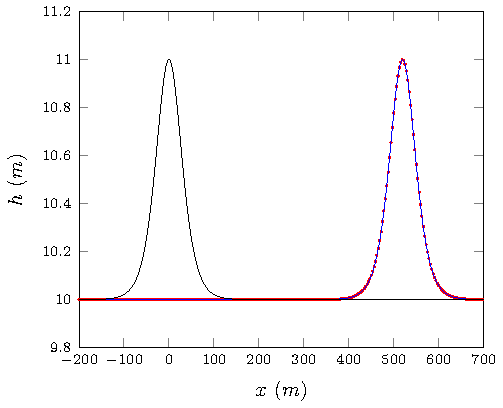
\includegraphics[width=5.0cm]{../pictures/soliton/lownonling10/ex/o2plotsolh-figure0.pdf}
%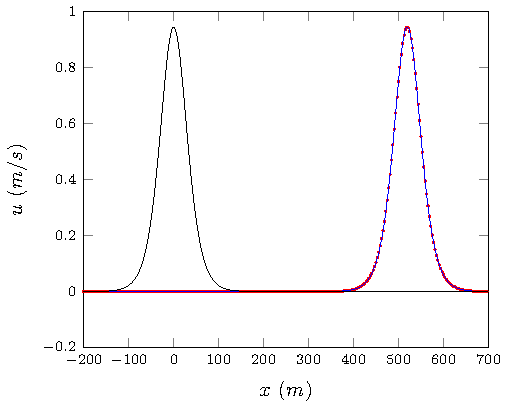
\includegraphics[width=5.0cm]{../pictures/soliton/lownonling10/ex/o2plotsolu-figure0.pdf}
%\end{figure}
%\end{frame}

%\begin{frame}{Experiment 1}
%Third Order:

%\begin{figure}
%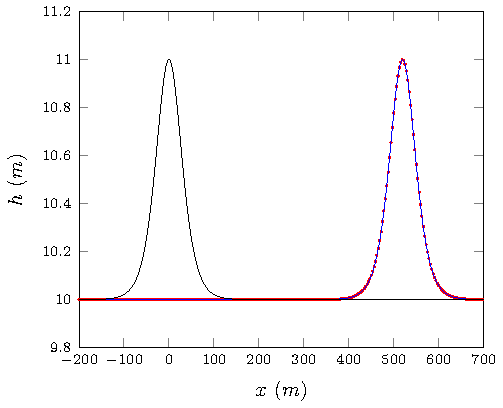
\includegraphics[width=5.0cm]{../pictures/soliton/lownonling10/ex/o2plotsolh-figure0.pdf}
%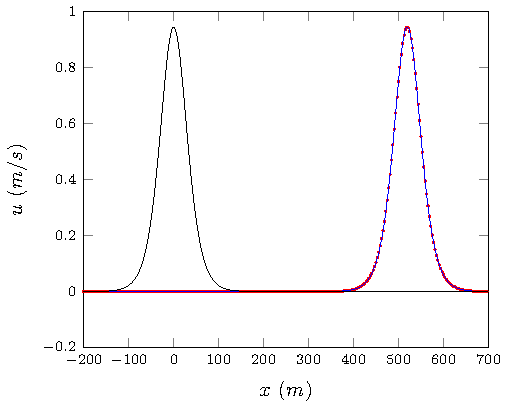
\includegraphics[width=5.0cm]{../pictures/soliton/lownonling10/ex/o2plotsolu-figure0.pdf}
%\end{figure}
%\end{frame}

%\begin{frame}{Experiment 1}
%Convergence

%\begin{figure}
%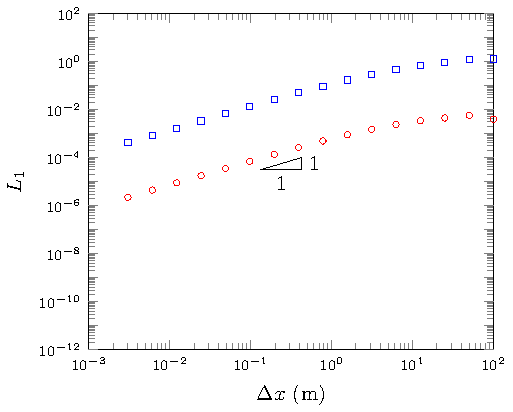
\includegraphics[width=3.9cm]{../pictures/soliton/lownonling10/con/sto1-figure0.pdf}
%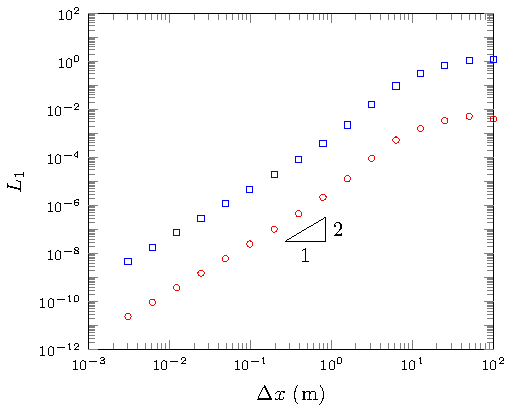
\includegraphics[width=3.9cm]{../pictures/soliton/lownonling10/con/sto2-figure0.pdf}
%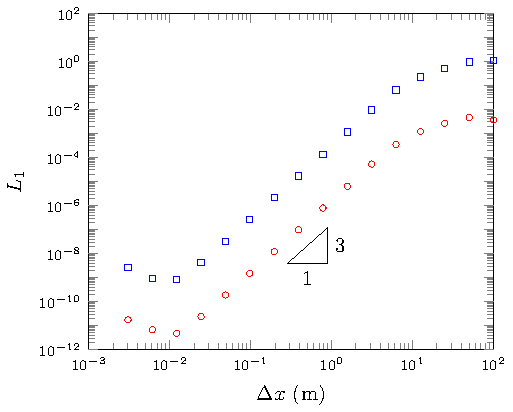
\includegraphics[width=3.9cm]{../pictures/soliton/lownonling10/con/sto3-figure0.pdf}
%\end{figure}
%\end{frame}

\begin{frame}{Experiment 1}
$a_0 = 1.0\text{m}$ , $a_1 = 1.0\text{m}$ ($\eta = 1.0$) , $\Delta x = 100 /2^{12}\text{m}$ , $\Delta t = \frac{0.5}{\sqrt{g (a_0 + a_1)}} \Delta x \; \text{s}$

First Order:

\begin{figure}
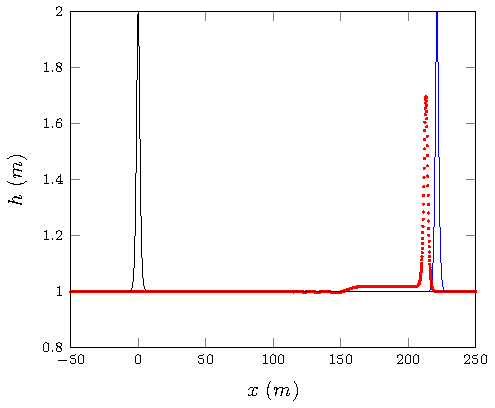
\includegraphics[width=5.0cm]{../pictures/soliton/hinonling10/ex/o1/12/plotsolh-figure0.pdf}
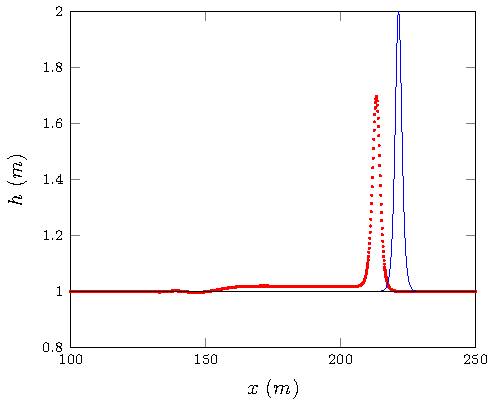
\includegraphics[width=5.0cm]{../pictures/soliton/hinonling10/ex/o1/12/plotsolhz-figure0.pdf}
\end{figure}
\end{frame}

\begin{frame}{Experiment 1}
Second Order:

\begin{figure}
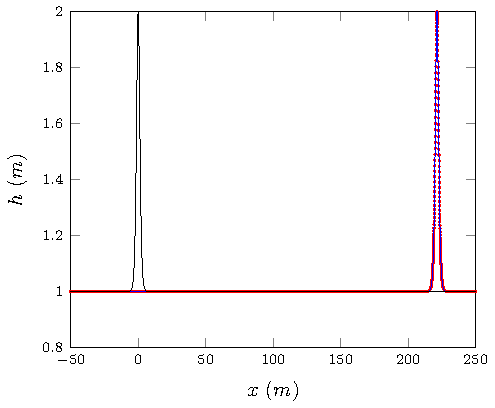
\includegraphics[width=5.0cm]{../pictures/soliton/hinonling10/ex/o2/12/plotsolh-figure0.pdf}
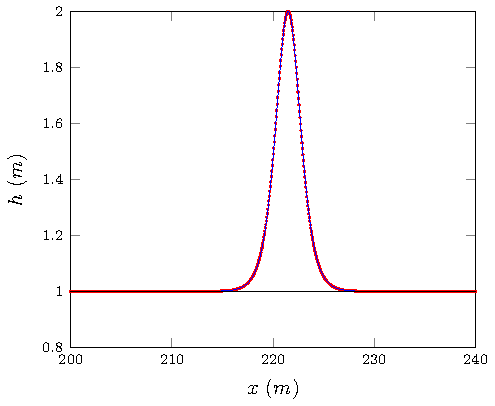
\includegraphics[width=5.0cm]{../pictures/soliton/hinonling10/ex/o2/12/plotsolhz-figure0.pdf}
\end{figure}
\end{frame}

\begin{frame}{Experiment 1}
Third Order:

\begin{figure}
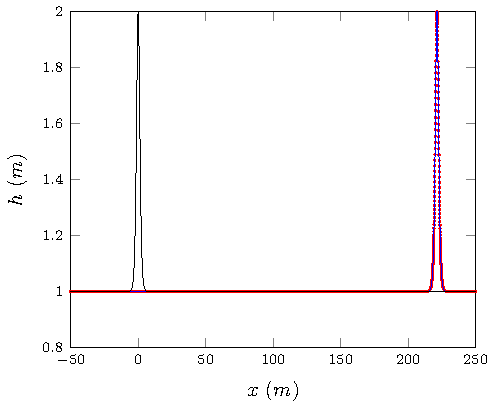
\includegraphics[width=5.0cm]{../pictures/soliton/hinonling10/ex/o3/12/plotsolh-figure0.pdf}
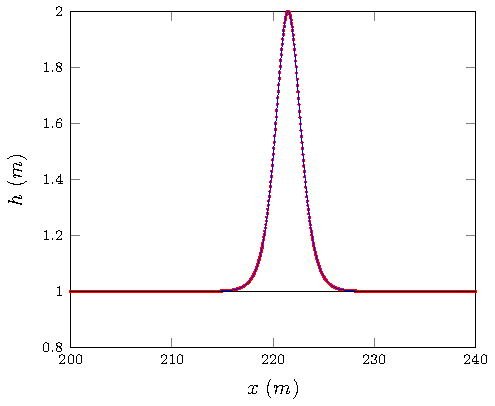
\includegraphics[width=5.0cm]{../pictures/soliton/hinonling10/ex/o3/12/plotsolhz-figure0.pdf}
\end{figure}
\end{frame}

\begin{frame}{Experiment 1}
Convergence:

\begin{figure}
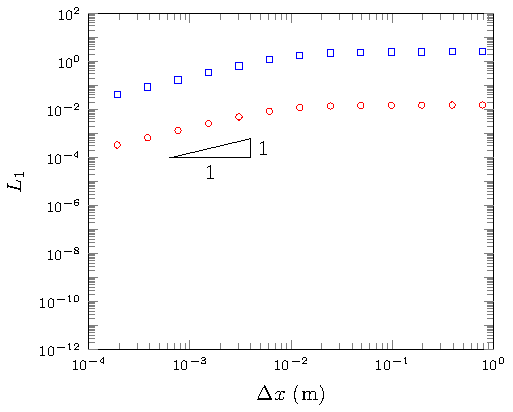
\includegraphics[width=3.9cm]{../pictures/soliton/hinonling10/con/sto1-figure0.pdf}
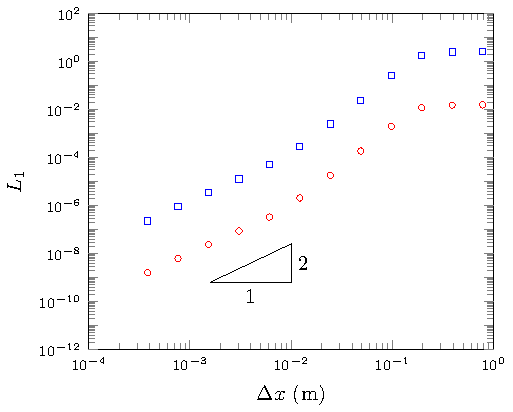
\includegraphics[width=3.9cm]{../pictures/soliton/hinonling10/con/sto2-figure0.pdf}
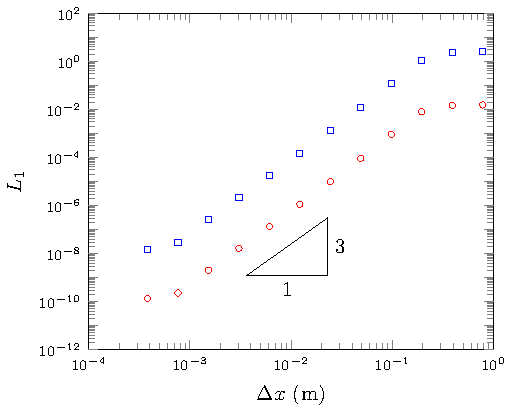
\includegraphics[width=3.9cm]{../pictures/soliton/hinonling10/con/sto3-figure0.pdf}
\end{figure}
\end{frame}


\subsection{Experimental Validation}

\begin{frame}{Hammack and Segur}
\begin{figure}
\cite{Hammack-Segur-1978-337}
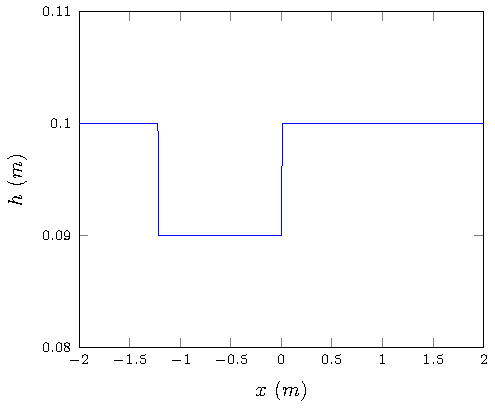
\includegraphics[width=7cm]{../pictures/added/hs2.pdf}
\end{figure}
\end{frame}

\begin{frame}{Segur and Hammack}
$\Delta x = 0.1 \text{m}$ , $\Delta t = \frac{0.5}{\sqrt{g 0.1}} \Delta x \; \text{s}$ \\

First Order at $x = 10\text{m}$ and $x = 20 \text{m}$
\begin{figure}
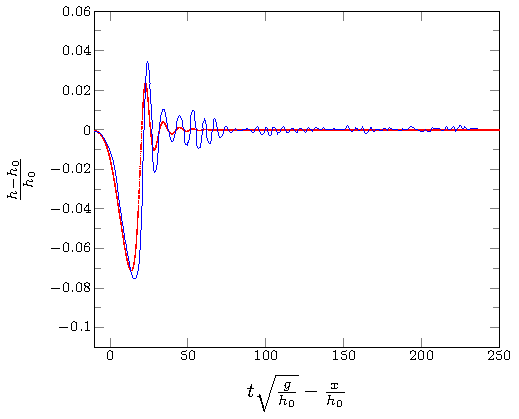
\includegraphics[width=5.5cm]{../pictures/segur/o1/plotp10-figure0.pdf}
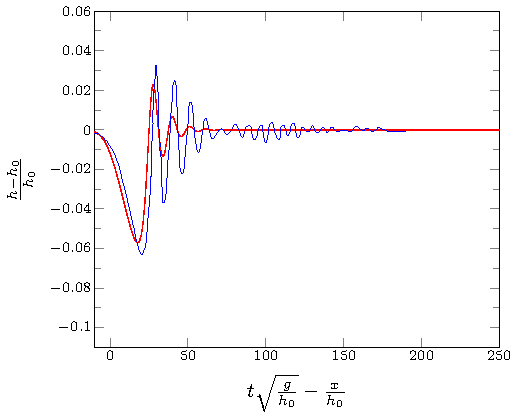
\includegraphics[width=5.5cm]{../pictures/segur/o1/plotp20-figure0.pdf}
\end{figure}
\end{frame}

\begin{frame}{Segur and Hammack}
Second Order at $x = 10\text{m}$ and $x = 20 \text{m}$
\begin{figure}
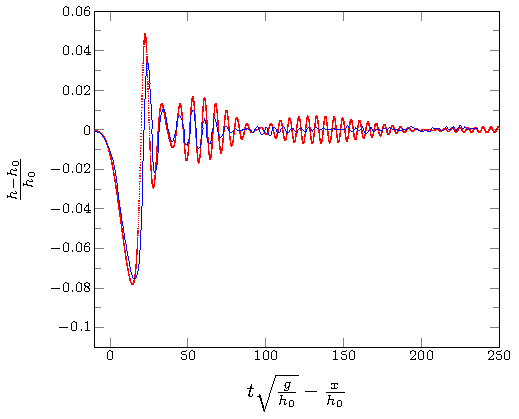
\includegraphics[width=5.5cm]{../pictures/segur/o2/plotp10-figure0.pdf}
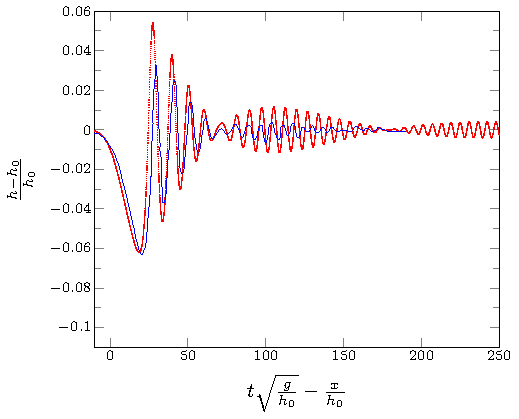
\includegraphics[width=5.5cm]{../pictures/segur/o2/plotp20-figure0.pdf}
\end{figure}
\end{frame}

\begin{frame}{Segur and Hammack}
Third Order at $x = 10\text{m}$ and $x = 20 \text{m}$
\begin{figure}
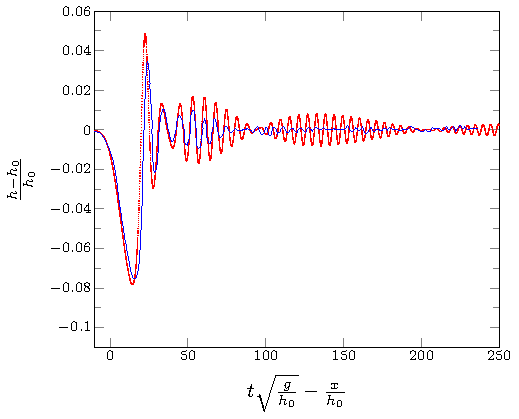
\includegraphics[width=5.5cm]{../pictures/segur/o3/plotp10-figure0.pdf}
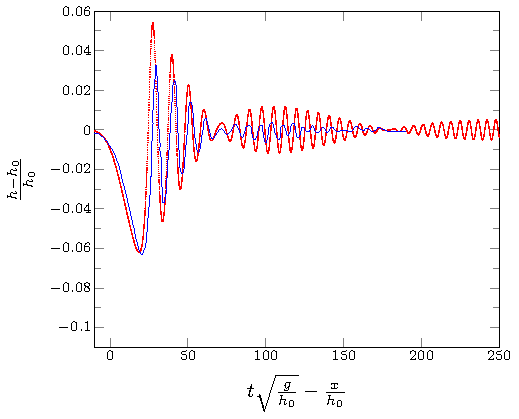
\includegraphics[width=5.5cm]{../pictures/segur/o3/plotp20-figure0.pdf}
\end{figure}
\end{frame}

\section{Smooth Dambreak}
\subsection{Description}

\begin{frame}{Plot}
$\Delta x = \frac{10}{2^6} \text{m}$
\begin{figure}
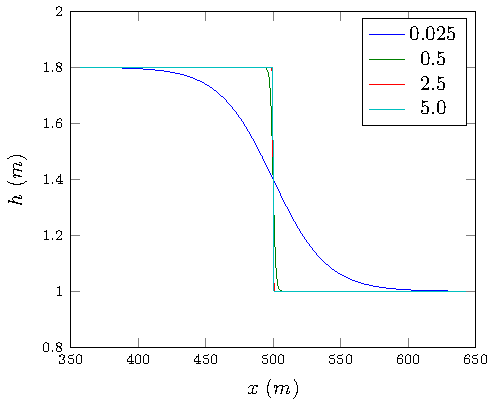
\includegraphics[width=7.5cm]{../pictures/added/db1.pdf}
\end{figure}
%\begin{figure}
%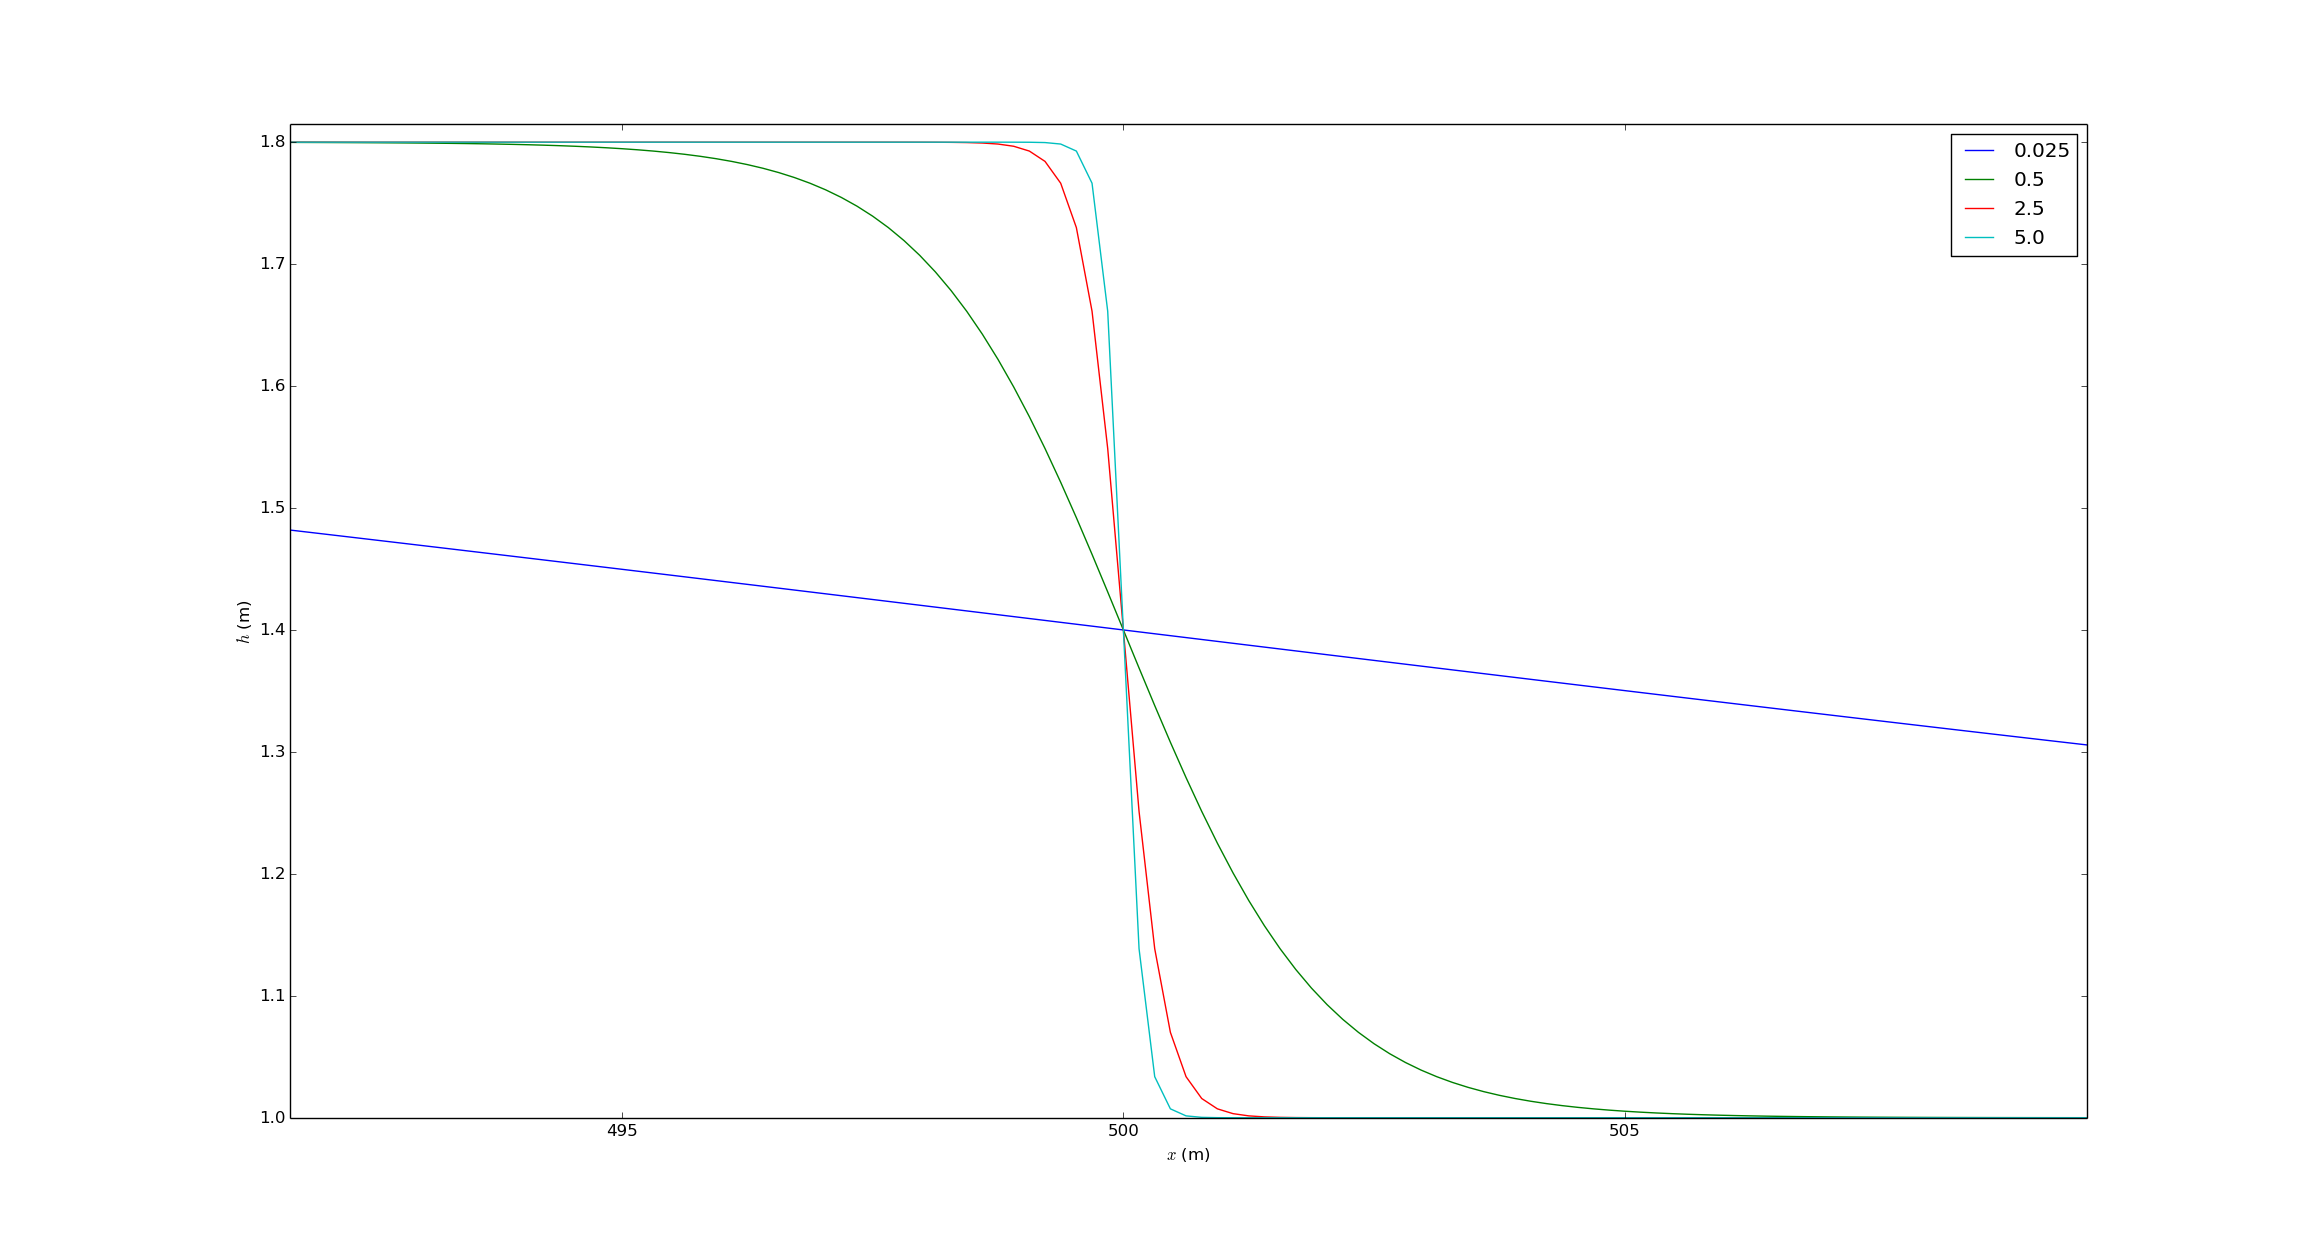
\includegraphics[width=6cm]{../pictures/added/figure_2.png}
%\end{figure}

\end{frame}

\begin{frame}{Equations}

\begin{subequations}
\begin{gather}
h(x,0) = h_0 + \frac{h_1 - h_0}{2}\left(1 + \tanh\left(\alpha\left(x_0 - x\right)\right)\right) \; \text{m},
\end{gather}
\begin{gather}
u(x,0) = 0.0 \text{m}/\text{s}.
\end{gather}
\end{subequations}
\label{eq:sdbi}

Problem of interest:
$h_0 = 1\text{m}$ , $h_1 = 1.8\text{m}$ , $x_0 = 500\text{m}$, $\Delta t = 0.01 \Delta x$
\end{frame}

\subsection{Varying $\Delta x$ Scenarios}

%\begin{frame}{Description}
%It was observed that by taking $\Delta x$ smaller and smaller for a wide array of $\alpha$ values that we can choose $\alpha$ such that it appears our solutions converge to four different scenarios.
%\end{frame}

\begin{frame}{No oscillations}
\begin{figure}
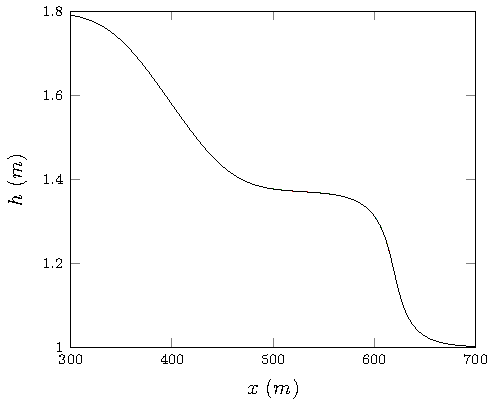
\includegraphics[width=7cm]{../pictures/smoothdambreak/dxto0/1diffmdx/paperpics/o3/1/nb3ne10/0-figure0.pdf}
%diffuses = [0.01,0.025,0.05,0.075,0.1,0.25,0.5,0.75,1.0,2.5,5.0,7.5,10.0,25.0,50.0,75.0,100.0,250.0,500.0,750.0,1000.0]
\end{figure}
$\alpha = 0.025$ and $\Delta x = \frac{10}{2^k}  \text{m}$ with $k = [3,4,\cdots,9]$
\end{frame}

\begin{frame}{Flat middle}
\begin{figure}
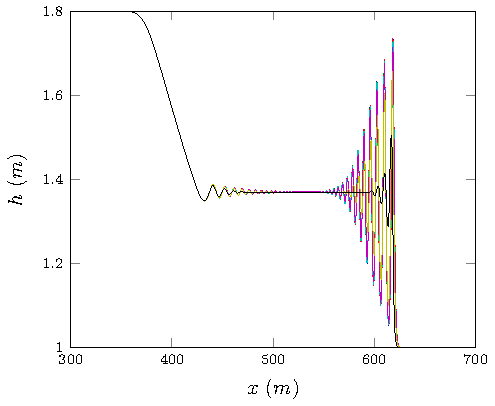
\includegraphics[width=7cm]{../pictures/smoothdambreak/dxto0/1diffmdx/paperpics/o3/6/nb3ne10/0-figure0.pdf}
%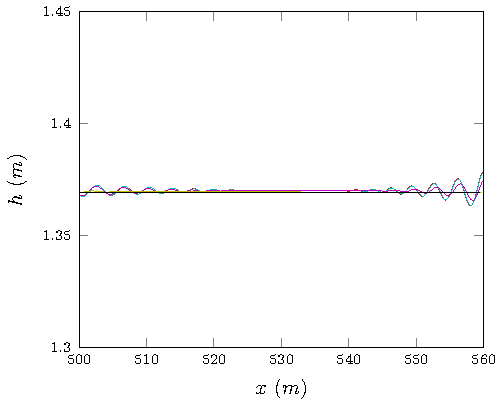
\includegraphics[width=5.5cm]{../pictures/smoothdambreak/dxto0/1diffmdx/paperpics/o3/6/nb3ne10/1-figure0.pdf}
%diffuses = [0.01,0.025,0.05,0.075,0.1,0.25,0.5,0.75,1.0,2.5,5.0,7.5,10.0,25.0,50.0,75.0,100.0,250.0,500.0,750.0,1000.0]
\end{figure}
$\alpha = 0.5$ and $\Delta x = \frac{10}{2^k} \text{m}$ with $k = [3,4,\cdots,9]$
\end{frame}

\begin{frame}{}
\begin{figure}
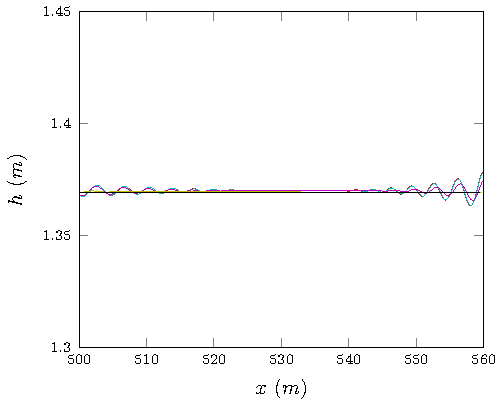
\includegraphics[width=7cm]{../pictures/smoothdambreak/dxto0/1diffmdx/paperpics/o3/6/nb3ne10/1-figure0.pdf}
\end{figure}
\cite{Hank-etal-2010-2034}
\end{frame}

\begin{frame}{Contact Discontinuity}
\begin{figure}
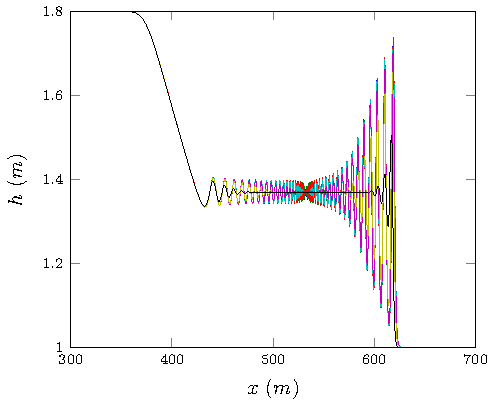
\includegraphics[width=7cm]{../pictures/smoothdambreak/dxto0/1diffmdx/paperpics/o3/9/nb3ne10/0-figure0.pdf}
\end{figure}
$\alpha = 2.5$ and $\Delta x = \frac{10}{2^k} \text{m}$ with $k = [3,4,\cdots,9]$
\end{frame}

\begin{frame}{}
\begin{figure}
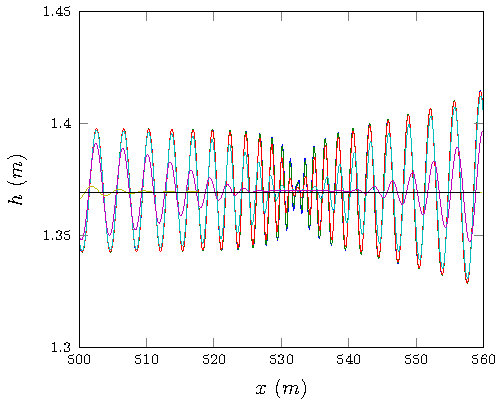
\includegraphics[width=7cm]{../pictures/smoothdambreak/dxto0/1diffmdx/paperpics/o3/9/nb3ne10/1-figure0.pdf}
\end{figure}
\cite{El-etal-2006}
\end{frame}

\begin{frame}{}
\begin{figure}
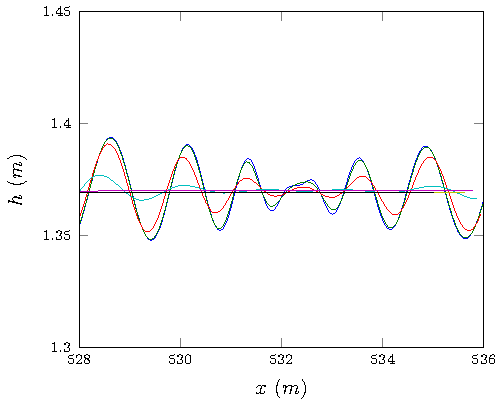
\includegraphics[width=9cm]{../pictures/smoothdambreak/dxto0/1diffmdx/paperpics/o3/9/nb3ne10/3-figure0.pdf}
\end{figure}
\end{frame}

\begin{frame}{Bump}
\begin{figure}
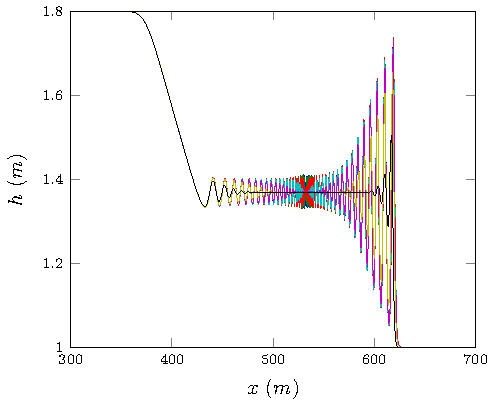
\includegraphics[width=7cm]{../pictures/smoothdambreak/dxto0/1diffmdx/paperpics/o3/10/nb3ne10/0-figure0.pdf}
\end{figure}
$\alpha = 5.0$ and $\Delta x = \frac{10}{2^k} \text{m}$ with $k = [3,4,\cdots,9]$
\end{frame}

\begin{frame}{}
\begin{figure}
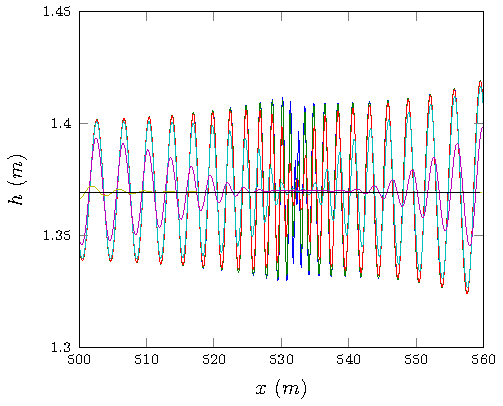
\includegraphics[width=9cm]{../pictures/smoothdambreak/dxto0/1diffmdx/paperpics/o3/10/nb3ne10/1-figure0.pdf}
\end{figure}
\end{frame}

\begin{frame}{}
\begin{figure}
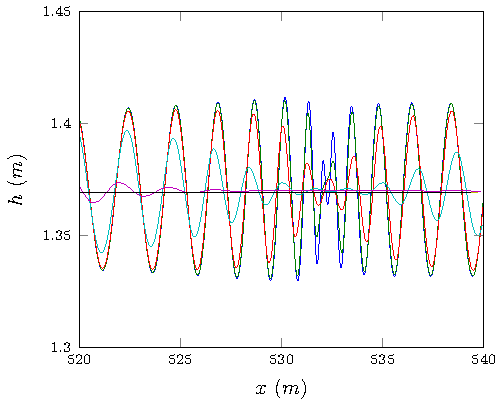
\includegraphics[width=9cm]{../pictures/smoothdambreak/dxto0/1diffmdx/paperpics/o3/10/nb3ne10/2-figure0.pdf}
\end{figure}
\end{frame}

\begin{frame}{Larger Bump}
\begin{figure}
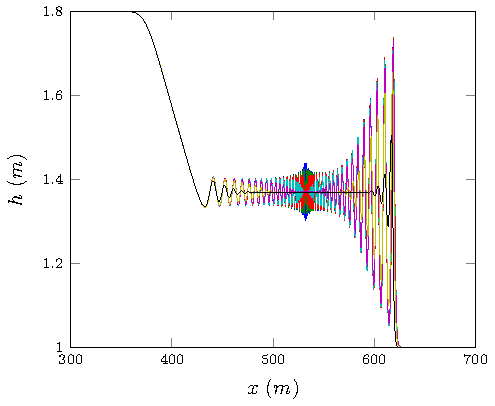
\includegraphics[width=7cm]{../pictures/smoothdambreak/dxto0/1diffmdx/paperpics/o3/20/nb3ne10/0-figure0.pdf}
\end{figure}
$\alpha = 1000$ and $\Delta x = \frac{10}{2^k} \text{m}$ with $k = [3,4,\cdots,9]$
\end{frame}

\begin{frame}{}
\begin{figure}
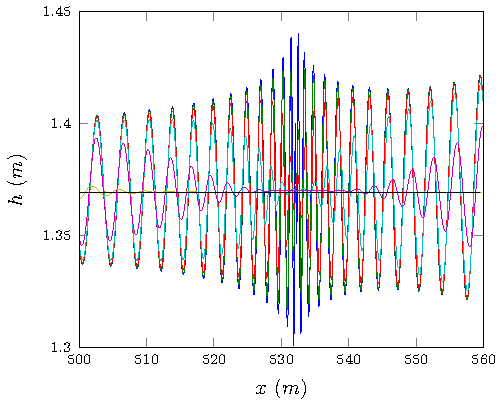
\includegraphics[width=9cm]{../pictures/smoothdambreak/dxto0/1diffmdx/paperpics/o3/20/nb3ne10/1-figure0.pdf}
\end{figure}
\end{frame}

\begin{frame}{}
\begin{figure}
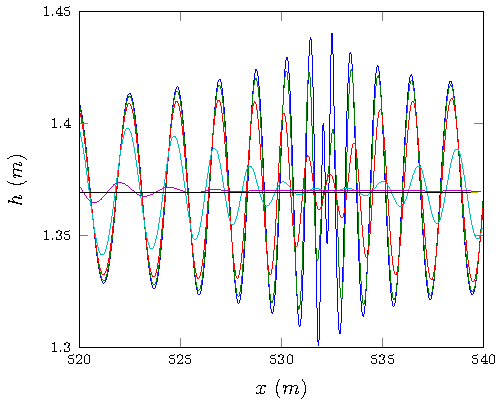
\includegraphics[width=9cm]{../pictures/smoothdambreak/dxto0/1diffmdx/paperpics/o3/20/nb3ne10/2-figure0.pdf}
\end{figure}
\end{frame}

\begin{frame}{Finite Difference Schemes}
Same results however very steep gradients cause problems
\begin{figure}
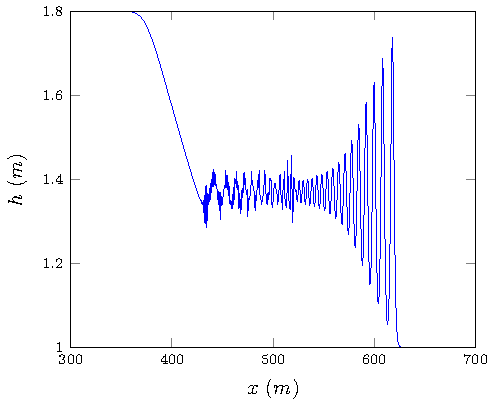
\includegraphics[width=6cm]{../pictures/smoothdambreak/dxto0/1diffmdx/nepics/examples/4/Joebigsmoothspec/FDcent/10/nbs4/1-figure0.pdf}
\end{figure}
$\alpha = 5.0$ $\Delta x = \frac{10}{2^4}\text{m} = 0.625\text{m}$
\end{frame}

\subsection{Changing $\alpha$}

\begin{frame}{Changing $\alpha$}
Can choose  $\Delta x$ such that as $\alpha$ gets larger our solutions converge to the same four scenarios as above.
\end{frame}

\section{References}
\begin{frame}[allowframebreaks]{References}
%--------------------------------------------------------------------------------
\bibliography{pres}
\bibliographystyle{apalike}
%--------------------------------------------------------------------------------
\end{frame}


\end{document}